\documentclass[12pt]{article}
\usepackage[a4paper, bindingoffset=0.2in, %
							left=0.5in,right=0.5in,top=0.5in,bottom=0.5in,%
							footskip=.25in]{geometry}
\usepackage{graphicx}
\usepackage{listings}
\usepackage{amssymb}
\usepackage{amsmath}
\usepackage{hyperref}


\title{PSet1 Report}
\author{Ali Abolhassanzadeh Mahani}
%\date{Oct. 15}

\begin{document}
	\maketitle
	\section{The Koch Fractal Set}
	\section{The Serpinski Fractal Set}
		\subsection{Deterministic}
		\subsection{Randomized}
	\section{Random Deposition}
	\subsection{Intro}
	In oder to work with Random Depostion, I made a function that generates the canvas,
	\texttt{n} times. This fucntion calls another function that generates the canvas
	\emph{once}. This, then, calls a function that deploys a particle using the rule that it's been
	given -- e.g. the Ballistic Deposition rule or the Competitve BD rule.
	
	\textbf{Equations to be used:}\\
	\emph{!! Note: $L$ is the length of the surface, $t$ is time, $w$ is width (roughness)}
	\begin{equation}
		w(L, t) = t^{\beta}, \, t \ll t_s
		\label{eq:beta}
	\end{equation}
	\begin{equation}
		t_s = L^z
		\label{eq:z}
	\end{equation}
	\begin{equation}
		w_s = t_s^\beta = L^{\beta z} = L^\alpha
		\label{eq:alpha}
	\end{equation}
	
	After generating the graphics once, I shutdown (\texttt{comment out}) the graphics part and do the calculations. I fit the curve using polyfit and reported the value for $\beta$
	\subsection{Random Deposition}
	The graphics to lay 25 layers is shown in Fig \ref{fig:RD25}
	\begin{figure}[h!]
		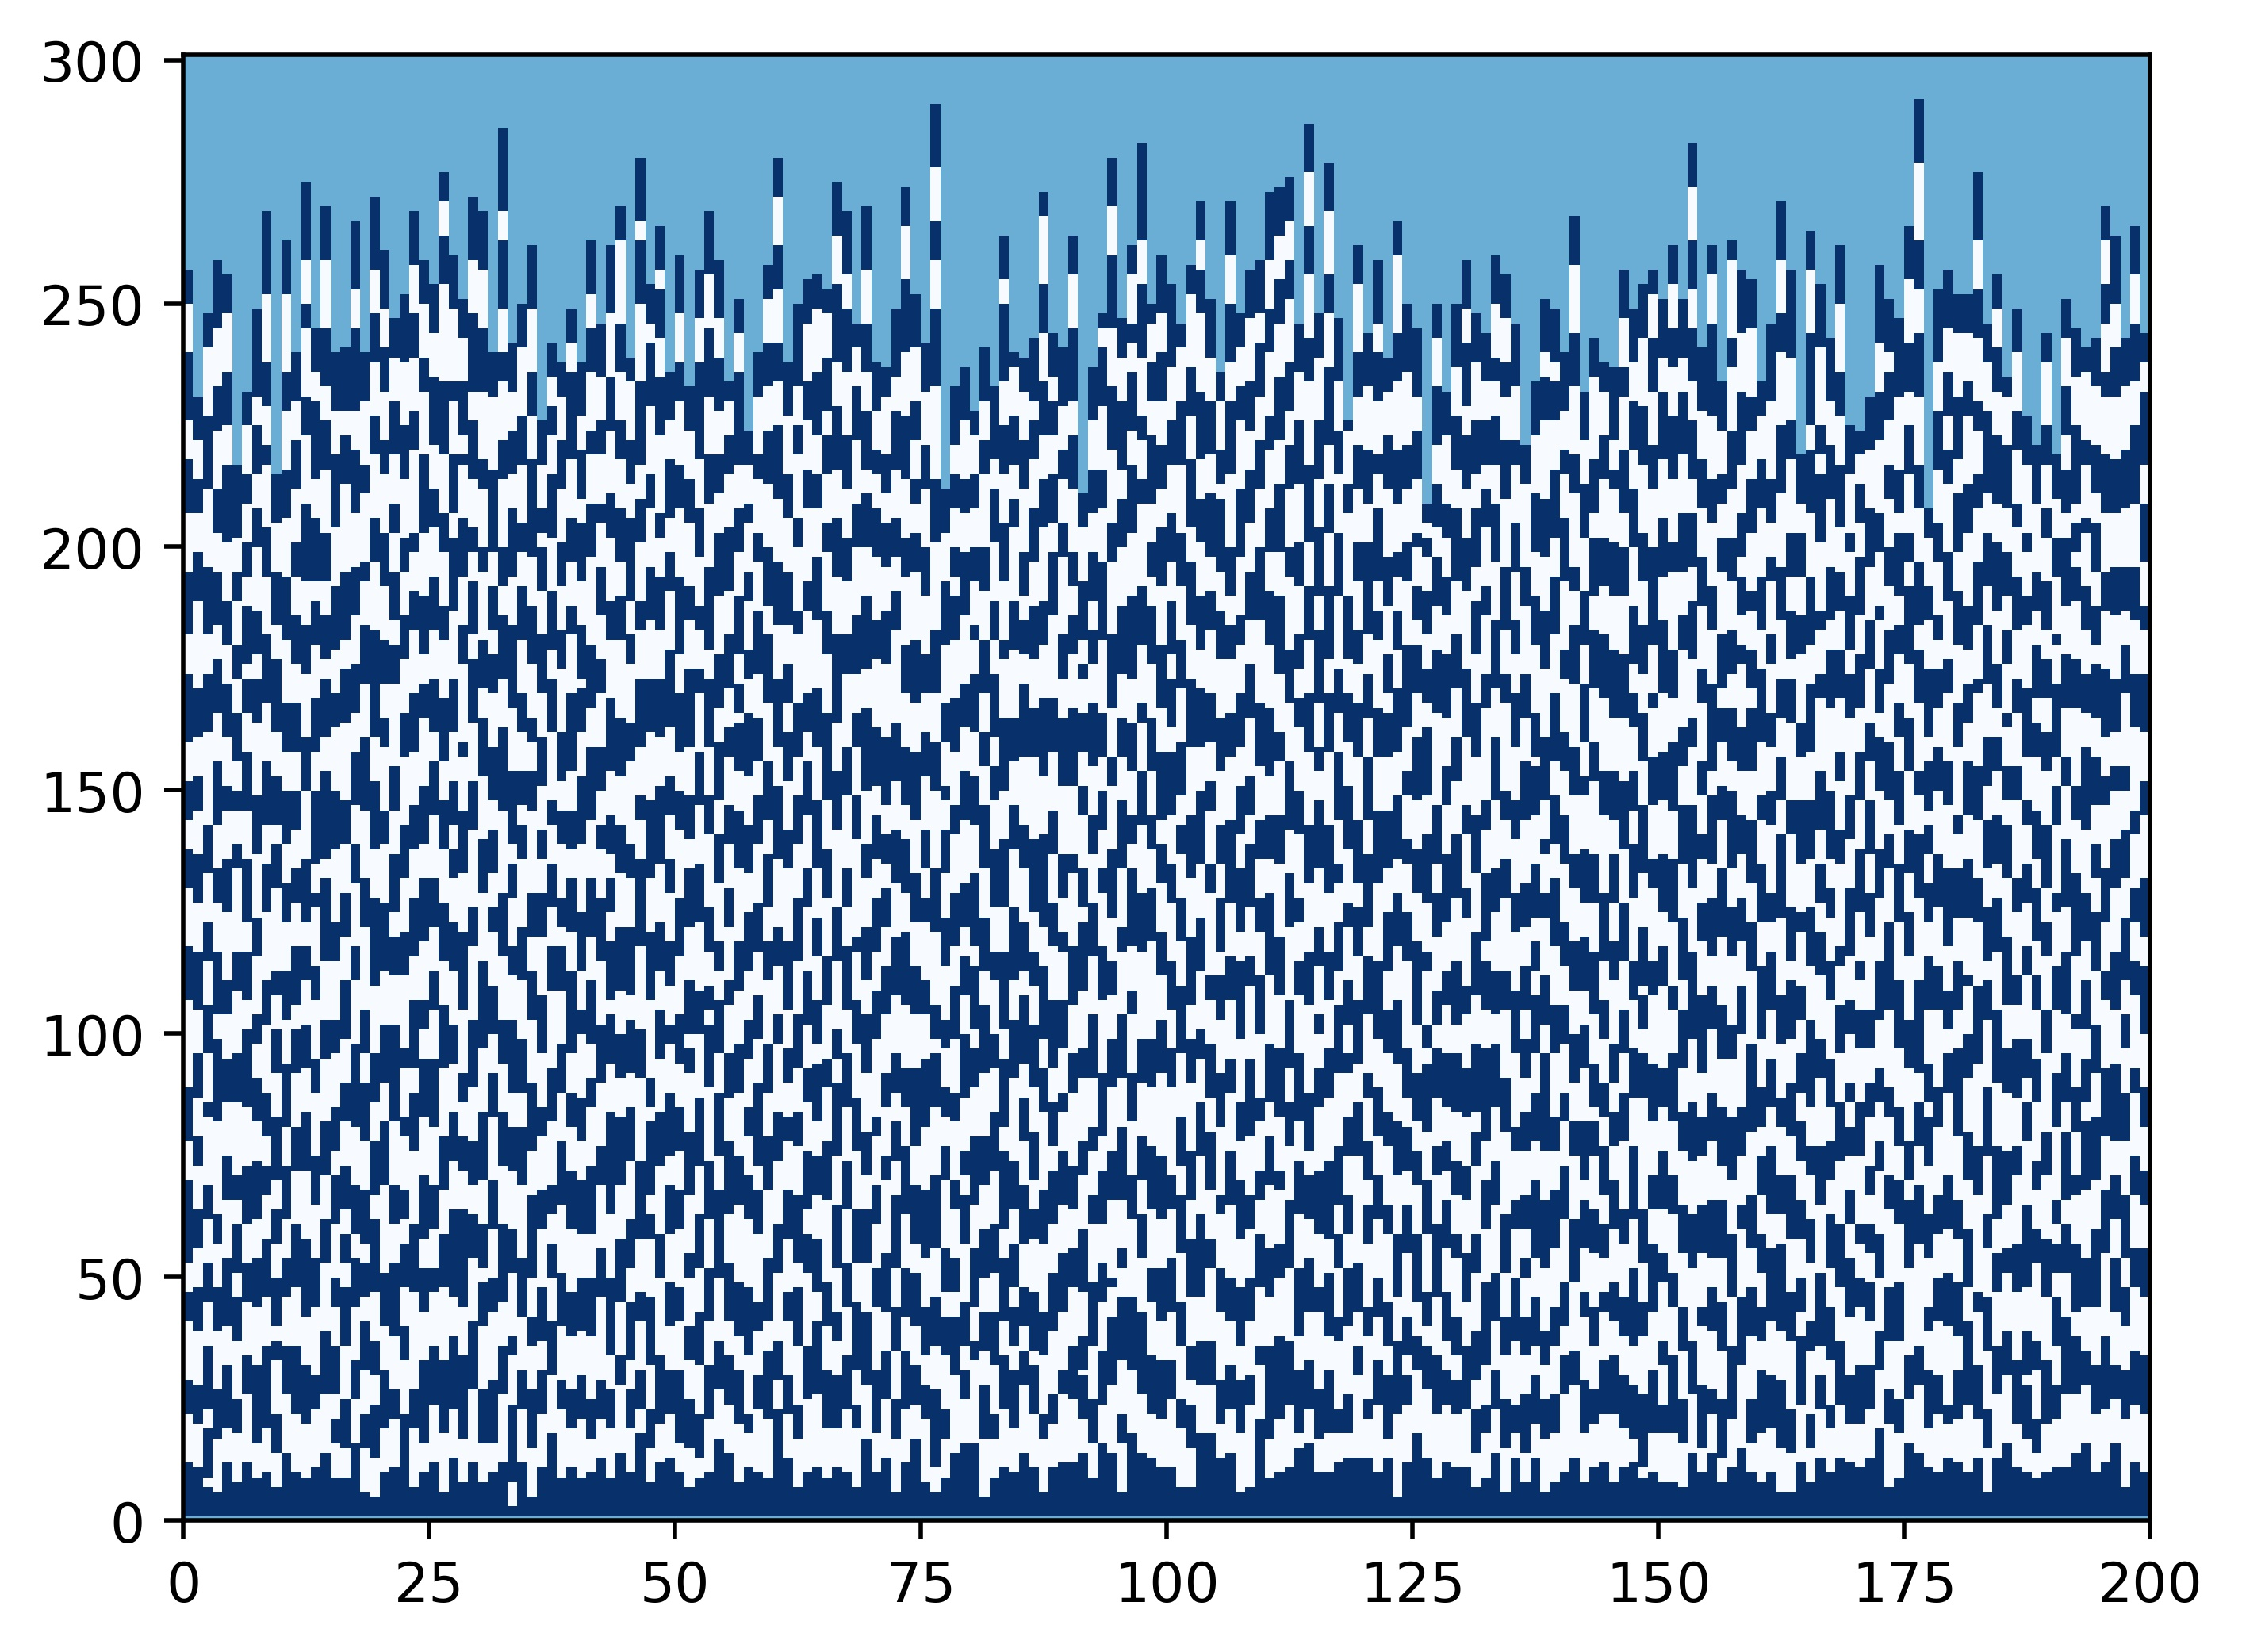
\includegraphics[width=\linewidth]{../P4/canvas.jpg}
		\label{fig:RD25}
		\caption{Randomly deposit particles on the surface of length 200 and change  color every 2000 particles you deposit. Do this for 50000 particles}
	\end{figure}
	The value for $\beta$ using eq.\ref{eq:beta} is as follows:
	\begin{equation*}
		\beta = 0.44 \pm 0.02
	\end{equation*}
	And the plot is shown at Fig.\ref{fig:RD25beta}
	\begin{figure}[h!]
		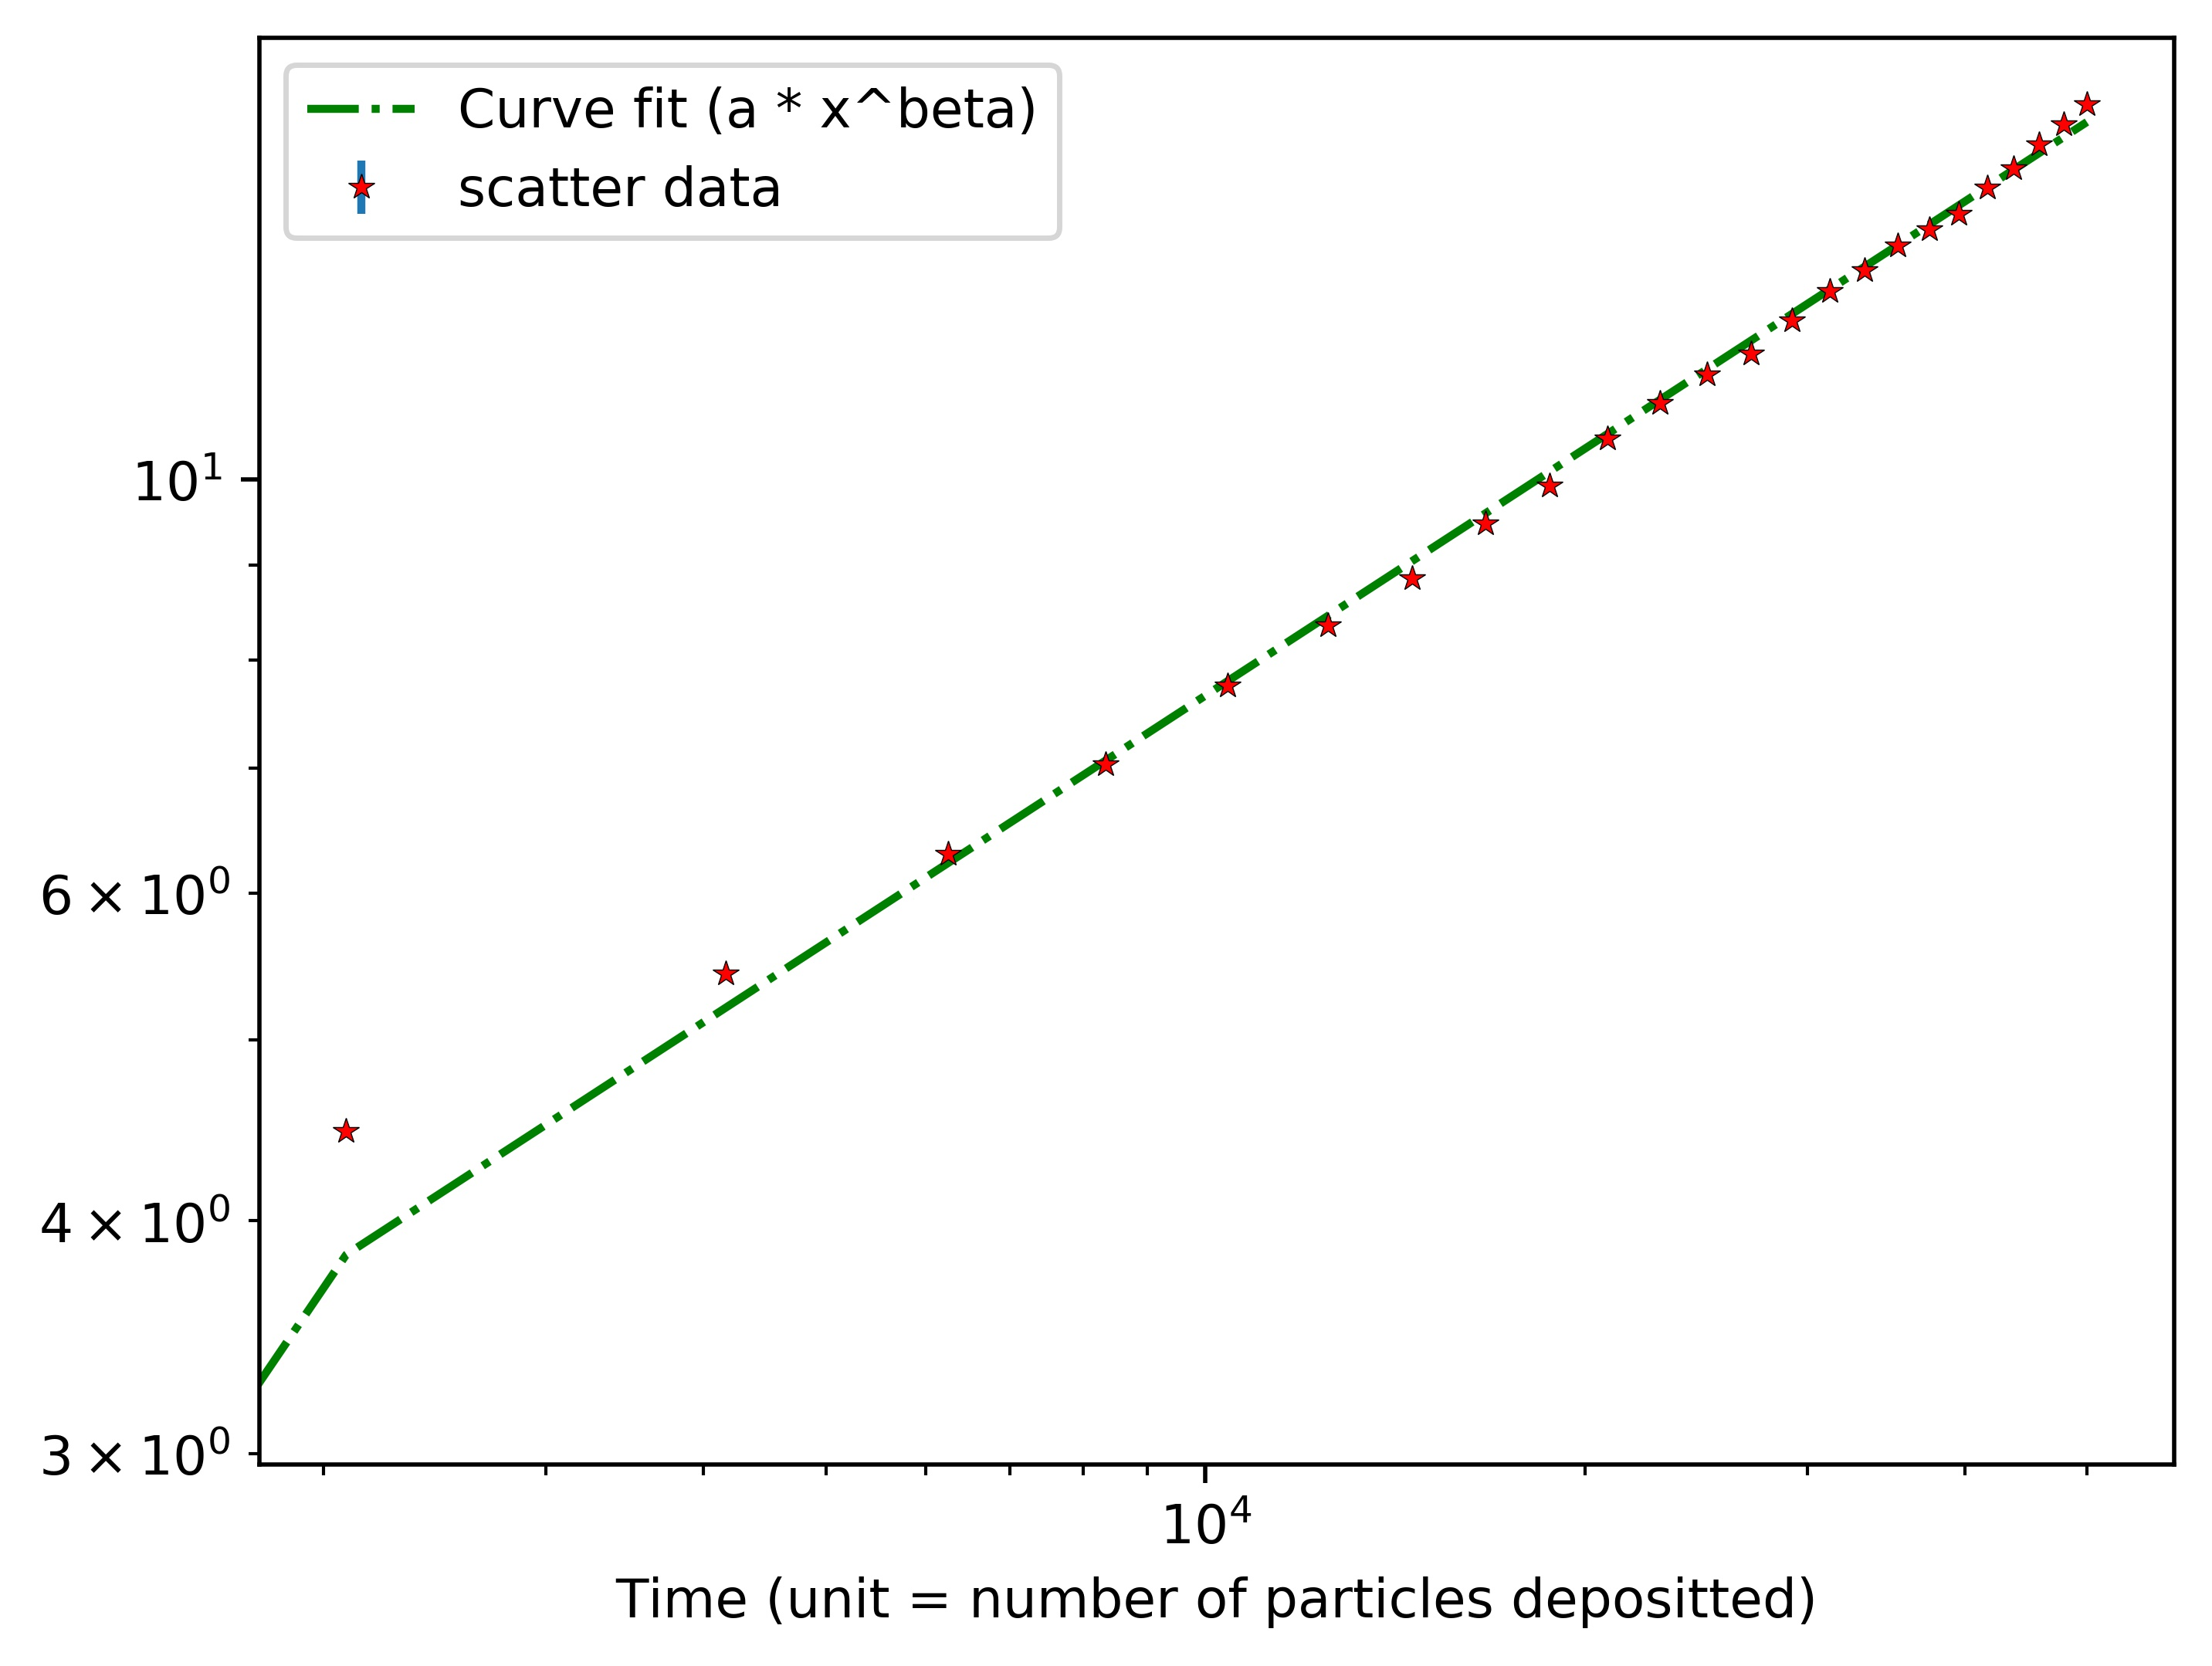
\includegraphics[width=\linewidth]{../P4/plot_for_beta.jpg}
		\label{fig:RD25beta}
		\caption{Take the stdev of height as roughness ($w(L, t)$) for every layer you deposit.
		do this 10 times and find the error of each layer. Then plot and fit using 
		\texttt{plt.errorbar} and \texttt{scipy.optimize.curve\_fit} respectively.}
	\end{figure}
	\subsection{Random Deposition with Surface Relaxation}
	The canvas for this part is shown in Fig\ref{fig:RDSR}.
	\begin{figure}[h!]
		\centering
		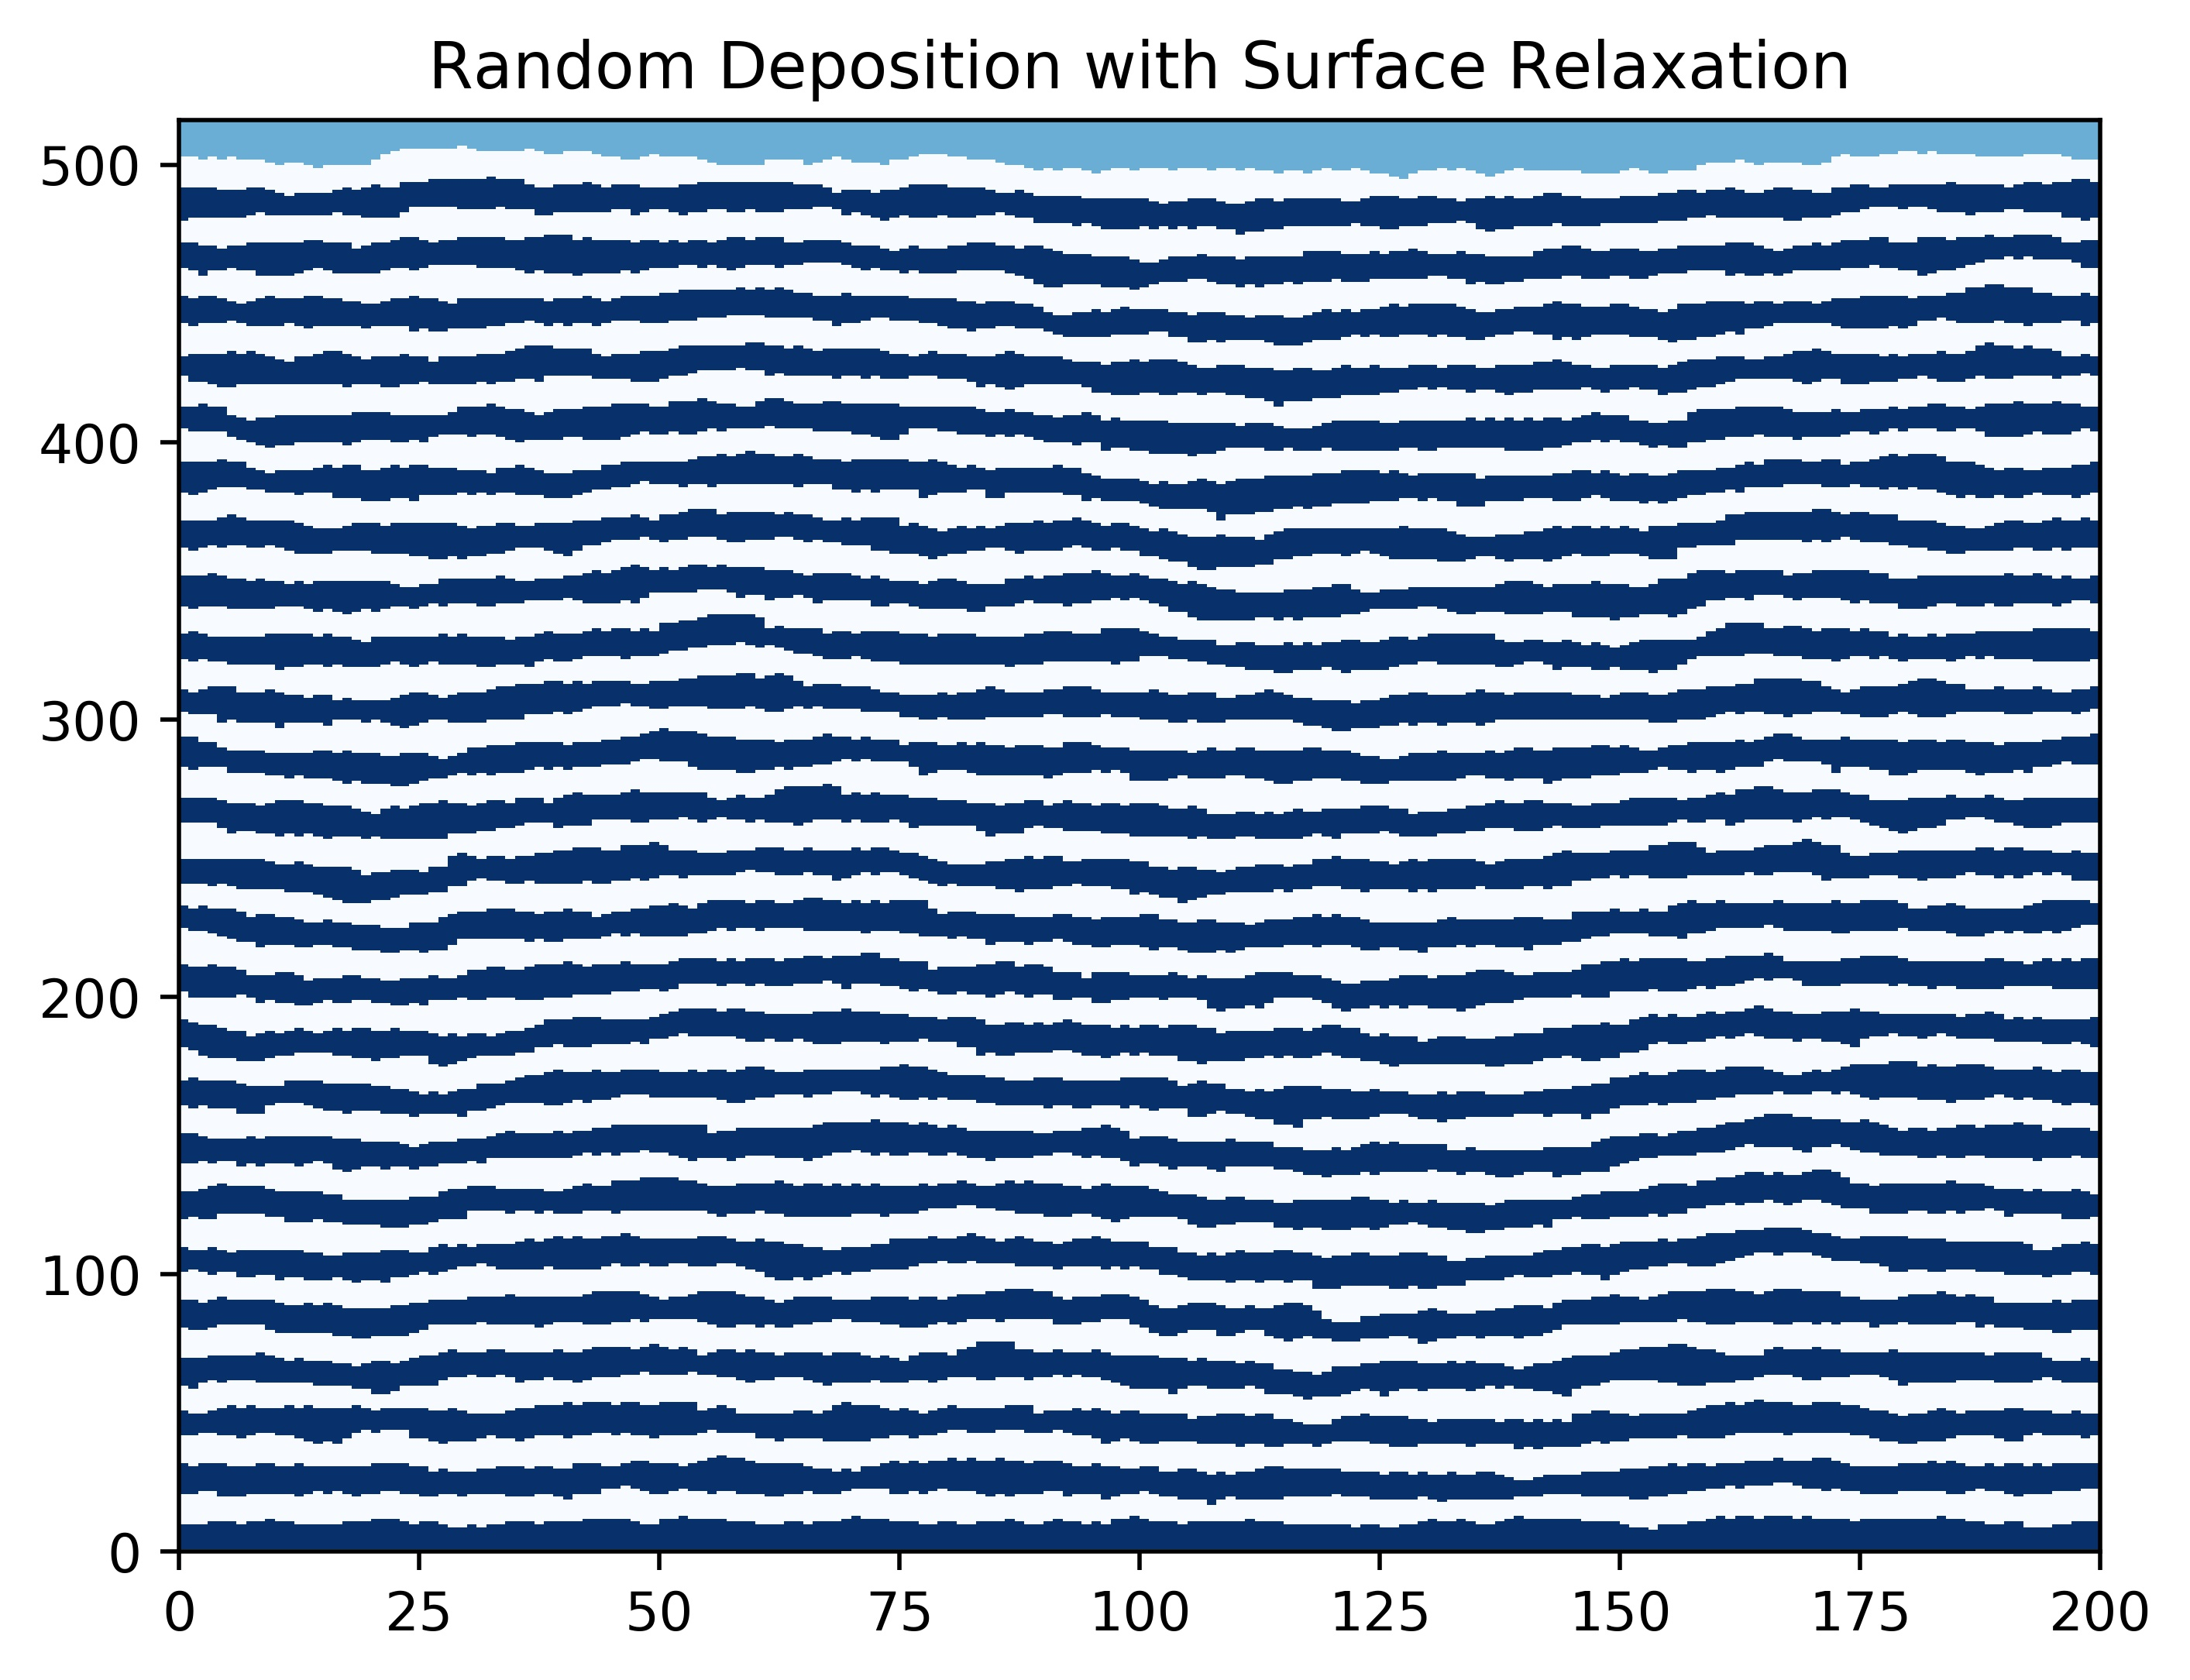
\includegraphics[width=.9\linewidth]{../P5/canvas.jpg}
		\label{fig:RDSR}
		\caption{deposit 100000 particles using the RDSR rule and output the data.}
	\end{figure}
	In order to reach saturation we need
	at least about 50000 particles. to make the plot (Fig\ref{fig:RDSRplot}) I ran the simulation 10 times with 800
	layer deposits total. The value for $t_s$ was output by looking at the graph and getting
	the data that was closest to the values we were looking for.
	The value found for beta is:
	\begin{figure}[h!]
		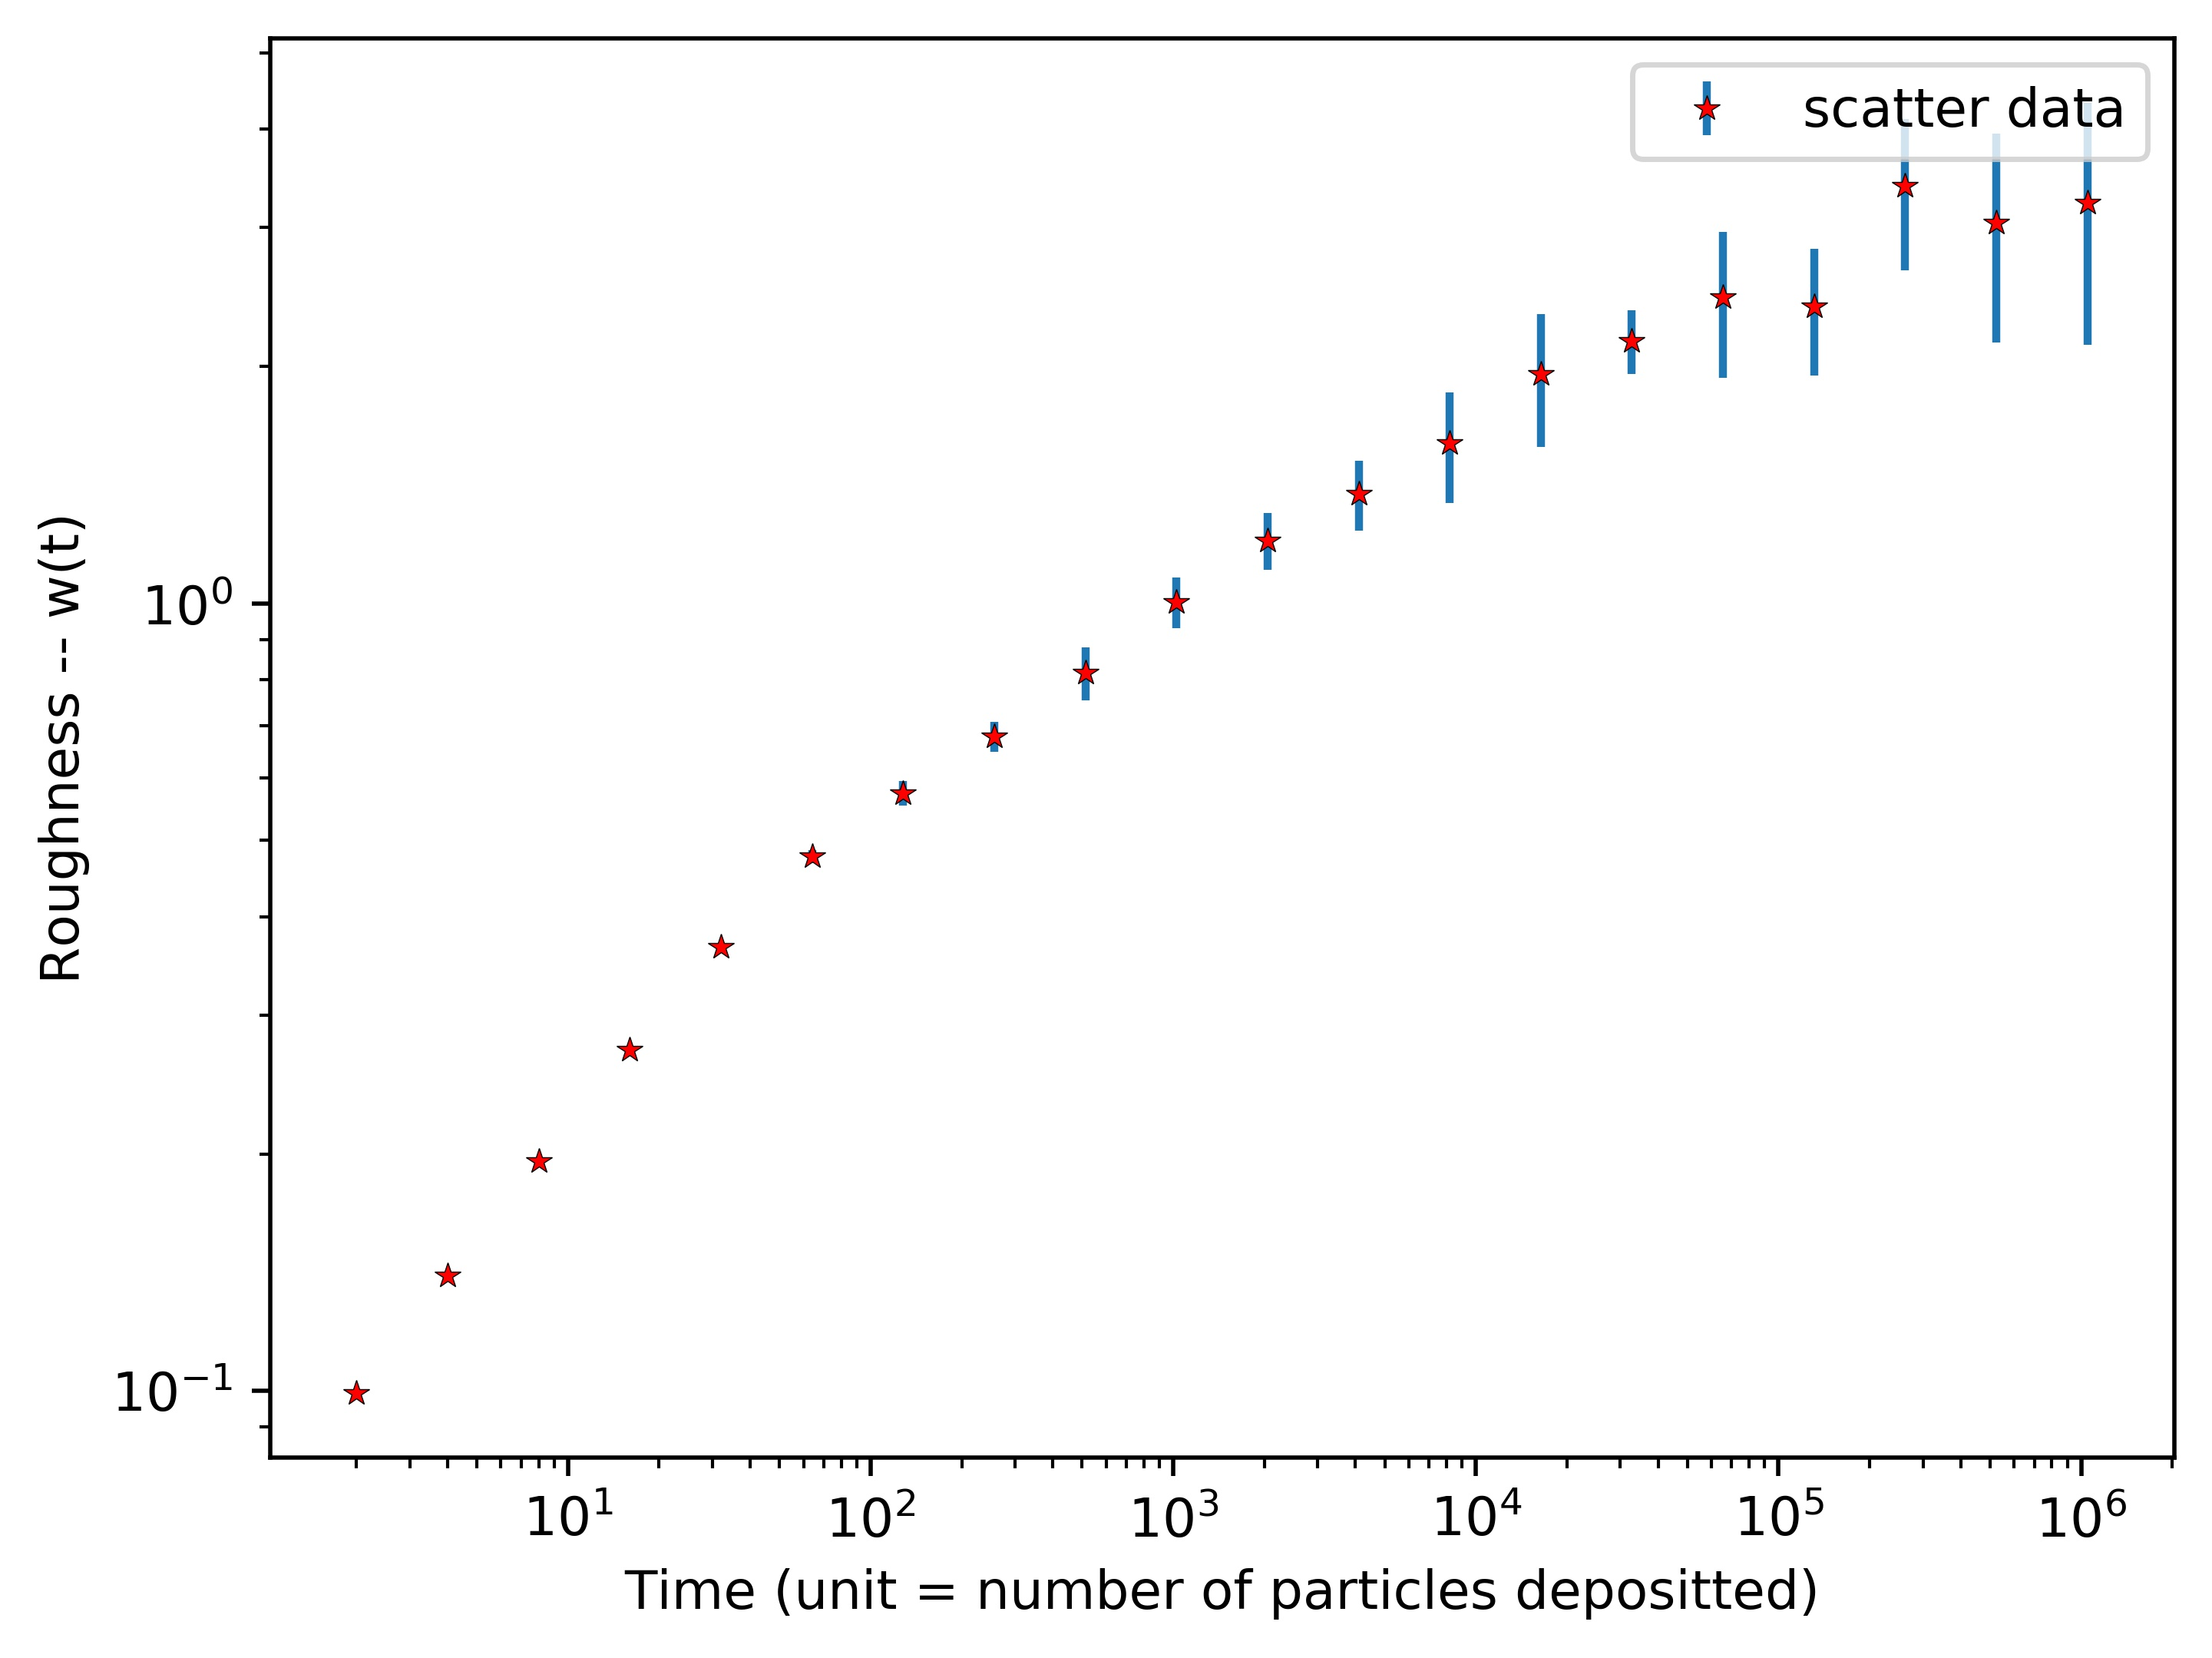
\includegraphics[width=0.9\linewidth]{../P5/plot_for_beta.jpg}
		\label{fig:RDSRplot}
		\caption{Plot log-log of roughness over time for RDSR}
	\end{figure}
	\begin{equation*}
		\beta = 1.64 \pm 0.06
	\end{equation*}
	The values for length $L$, saturation width $w_s$ and saturation time $t_s$ is as follows:
	\begin{equation*}
		\begin{aligned}
			L		 &= [10, 50, 100, 150, ]\\
			t_s		&= [32, 3072, 16384, 49152, 131072, 1048276]\\
			w_s	  &= [0.6, 1.1, 1.678, 2.725, 2.789, 3.558] 
		\end{aligned}
	\end{equation*}
	
	These values are plotted using the file \texttt{plots.py}. Plot fittings also happen there.
	
	Values found for $beta$ and $z$ are as follows:
	\begin{equation*}
		\beta = 0.18 \pm 0.02, \qquad z = 2.97 \pm 0.24, \qquad \Rightarrow \alpha \simeq 16.16
	\end{equation*}
	plots for $beta$ and $z$ are found in Fig\ref{fig:beta_z}
	\begin{figure}[h!]
		\centering
		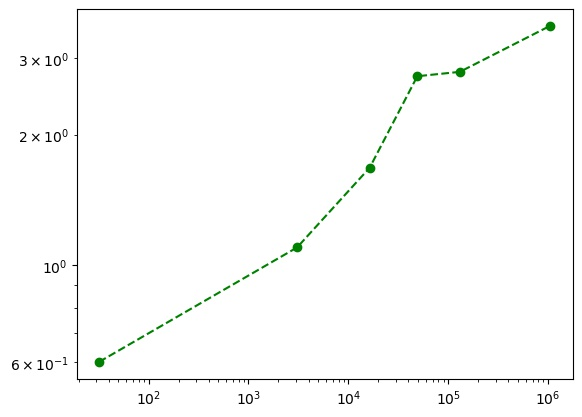
\includegraphics[width=.4\linewidth]{../P5/beta.jpg}
		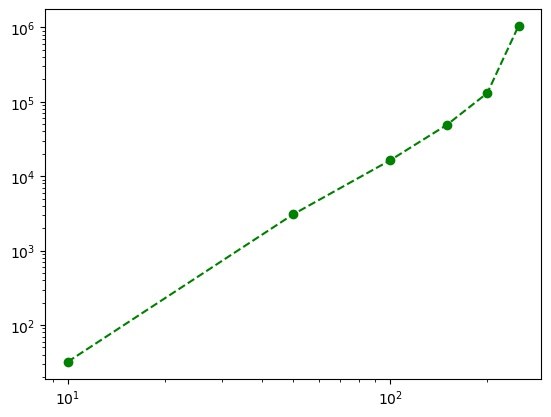
\includegraphics[width=.4\linewidth]{../P5/z.jpg}
		\label{fig:beta_z}
		\caption{The left log-log plot is for $w_s$ over $t_s$ and the one on the right is for 
		$t_s$ over length$L$. These plots are to measure $beta$, $z$ and $alpha$ in RDSR}
	\end{figure}
	
	\subsection{Ballistic Deposition}
	
	\subsection{Competitive Ballistic Deposition}
\end{document}